%%%%%%%%%%%%%%%%%%%%%%%%%%%%%%%%%%%%%%%%%%%%%%%%%%%%%%%%%%%%%%%%
%%                          CHAPTER 2                         %%
%%%%%%%%%%%%%%%%%%%%%%%%%%%%%%%%%%%%%%%%%%%%%%%%%%%%%%%%%%%%%%%%
\chapter{The synchroniser compiler}
  \section{Mathematical Model}
Synchroniser $S = (\Phi, \; \Pi)$, where
  \begin{itemize}
  \item[] $\Phi = (A, \; S, \; T)$ -- nondeterministic state machine:
    \begin{itemize}
    \item[] $A \subseteq C \times P$ -- the alphabet of events, $C$ -- set of synchroniser input channels, $P$ -- set of predicates on channel messages. An event $(c, \; p) \in A$ represents the reception of a message on channel $c$ that satisfies predicate $p$,
    \item[] $S \supseteq \{s_{0}\}$ -- set of abstract states, $s_{0}$ -- start state,
    \item[] $T \: : \: A \times S \to S$ -- transition matrix.
    \end{itemize}
  \item[] $\Pi \: : \: S \times \Omega \to V$ -- path functional that defines the synchroniser output:
    \begin{itemize}
    \item[] $\Omega$ -- the set of output channels,
    \item[] $V$ -- the set of message values \cite{astrakahn}.
    \end{itemize}
  \end{itemize}

In a state $s_{k}$ the functional is based on the retrospective sequence of transitions from the most recent visit to the start state $s_{0}$ to $s_{k}$:
  \begin{itemize}
  \item[] $(s_{0}, c_{0}), \: (s_{1}, c_{1}),... \: (s_{k}, c_{k})$, where
    \begin{itemize}
      \item[] $s_{0}$ -- start state,
      \item[] $c_{i} \in C$, $0 \le i \le k$ -- the channel that caused the transition from the state $s_{i}$.
    \end{itemize}
  \end{itemize}

Let $\mu_{i}$ be the message received in the transition from the state $s_{i}$. Then
  \begin{itemize}
  \item[] $\Pi \; (s_{k}, \omega_{m}) = \psi_{\sqcap} \; \{\mu_{i} \: | \: \rho_{ki}^{m} \; (s_{i}), \: 0 \le i \le k\}$, where
    \begin{itemize}
      \item[] $\rho_{ki}^{m}$ -- selection predicate that defines $\Pi$,
      \item[] $\psi_{\sqcap}$ -- the operator that coerces the messages in the operand set to their joint greatest subtype.
    \end{itemize}
  \end{itemize}

From the above, the synchroniser is fully defined by two functions:
  \begin{enumerate}
  \item The transition matrix $T$

The state machine can have a regular structure whereby many transitions can be defined at once by a formula with some limited range integer variables. For example, a machine with 8 states could have a transition matrix defined thus: $S_{k \; mod \; 8} \to S_{k+1 \; mod \; 8}$.

In order to be able to use regular structures, \ak\ allows synchronisers to declare \emph{state} variables.

\textbf{Example: the counter synchroniser}  Counter emits every $n$-th message received in its input channel to the output channel. The transition diagram for the counter synchroniser for $n = 3$ is given in Figure \ref{fig:counter}.a.

Mathematical model $S_{counter_{3}} = (\Phi, \; \Pi)$, where
  \begin{itemize}
  \item[] $\Phi = (A, \; S, \; T)$,
    \begin{itemize}
    \item[] $C = (a)$, $P = (true)$, $A = C \times P = ((a, \; true))$,
    \item[] $S = (s_{0}, \; s_{1}, \; s_{2})$, $s_{0}$ -- start state,
    \item[] $T$:
      \begin{tabular}{c|c|c|c}
      $A$ \textbackslash $S$ & $s_{0}$ & $s_{1}$ & $s_{2}$\\
      \hline
      $(a, \; true)$ & $s_{1}$ & $s_{2}$ & $s_{0}$\\
      \end{tabular}
    \end{itemize}
  \item[] $\Pi \: : \: S \times \Omega \to V$,
    \begin{itemize}
    \item[] $\Omega = (c)$,
    \item[] $V = (a)$
    \end{itemize}
  \end{itemize}

An output message is emitted when a transition happens from the state $s_{2}$. This state is reached in a single path:
  \begin{itemize}
  \item[]
$W_{0} = ((s_{0}, \; a), \: (s_{1}, \; a), \: (s_{2}, \; a))$
% fixed rho{1i}^{c} to rho{2i}^{c}
$\Pi \; (s_{2}, c) = \psi_{\sqcap} \; \{\mu_{0} = a \: | \: \rho_{20}^{c} \; (s_{0}) = 0, \mu_{1} = a \: | \: \rho_{21}^{c} \; (s_{1}) = 0, \mu_{2} = a \: | \: \rho_{22}^{c} \; (s_{2}) = 1\}$, $k = 1$, $i = 0,1,2$ 
  \end{itemize}

The state machine behind the counter has a regular structure, and for this synchroniser all its transitions may be defined with a single formula: $S_{k \; mod \; 3} \to S_{k+1 \; mod \; 3}$. Considering this, the transition matrix $T$ would be:
  \begin{tabular}{c|c}
  $A$ \textbackslash $S$ & $S_{k \; mod \; 3}$\\
  \hline
  $(a, \; true)$ & $S_{k+1 \; mod \; 3}$
  \end{tabular}

Some possible transition diagrams of the counter synchroniser are given in Figure \ref{fig:counter}. The diagram \ref{fig:counter}.a represents the unrolled regular structure of the synchroniser. However, this representation is inconvenient when $n \gg 1$. The transition diagram \ref{fig:counter}.a can be folded using state variables. Two possible variants are shown in figures \ref{fig:counter}.b and \ref{fig:counter}.c. The state variable $c$ acts as an induction variable in a while loop with the exit condition $c \ge 3$.

  \begin{figure}[here]
  \centering
  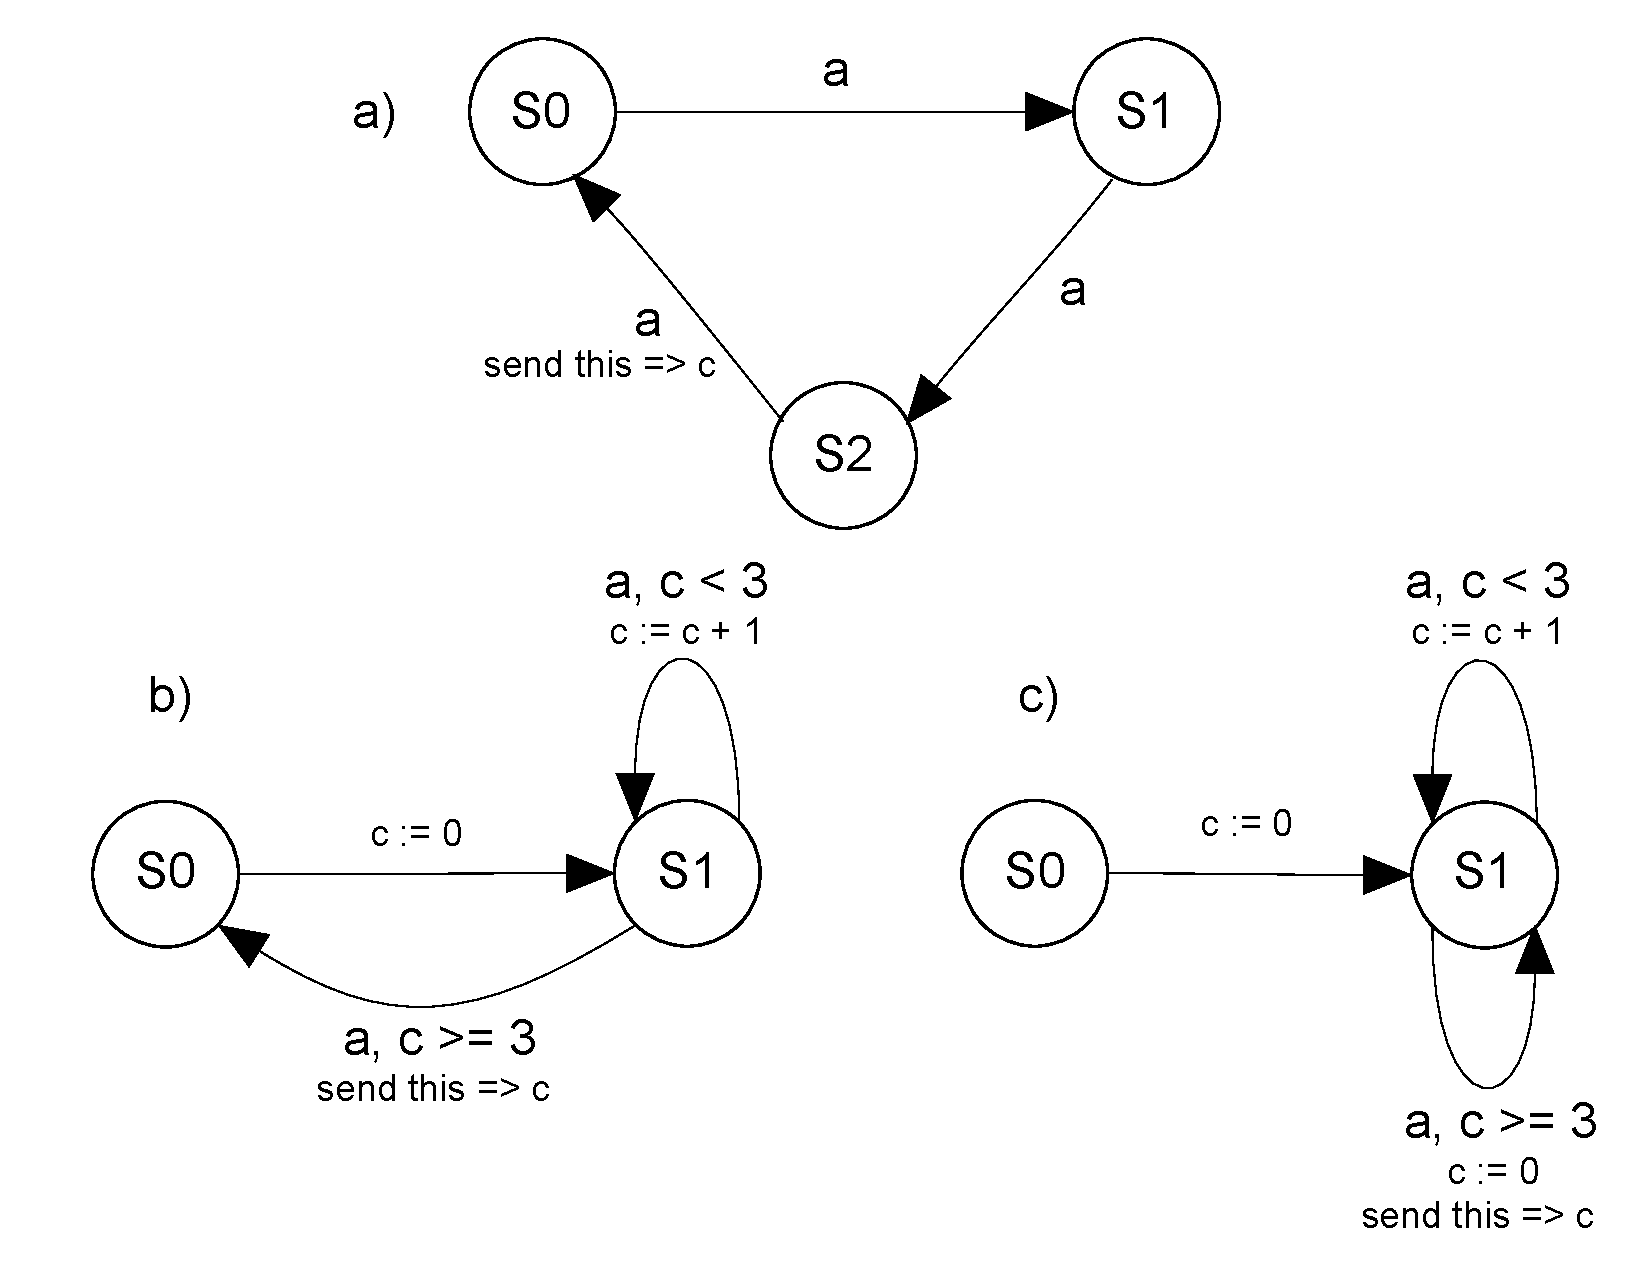
\includegraphics[scale=0.4]{figs/counter.pdf}
  \caption{The transition diagrams of the counter synchroniser.}
  \label{fig:counter}
  \end{figure}


  \item The selection predicate $\rho$

In a given state $k$ for each output channel $\omega_{m}$ we note all $i$ on which $\rho_{ki}^{m}$ is true. Those message values must be stored in a previous state and recalled in state $k$. It is expected that the boolean vector $\omega_{i} = \rho_{ki}^{m}$ has only very few true elements.

Consequently the storage mechanism that \ak\ provides for synchronisers is in the form of individual \emph{store} variables, which are associated with input channel types.

\textbf{Example: the binary zip synchroniser}  Zip2 receives messages on its input channels and sends their concatenation to the output channel. In the resulting concatenation there's exactly one message from each input channel and those messages are ordered as they received.

The zip2 transition diagram is given in Figure \ref{fig:zip2}. The message received in the current transition is referred by a keyword \emph{this}. $ma$ and $mb$ are the store variables associated with the input channels $a$ and $b$ respectively. The statement \emph{send} indicates a sending of a message to an output channel.

  \begin{figure}[here]
  \centering
  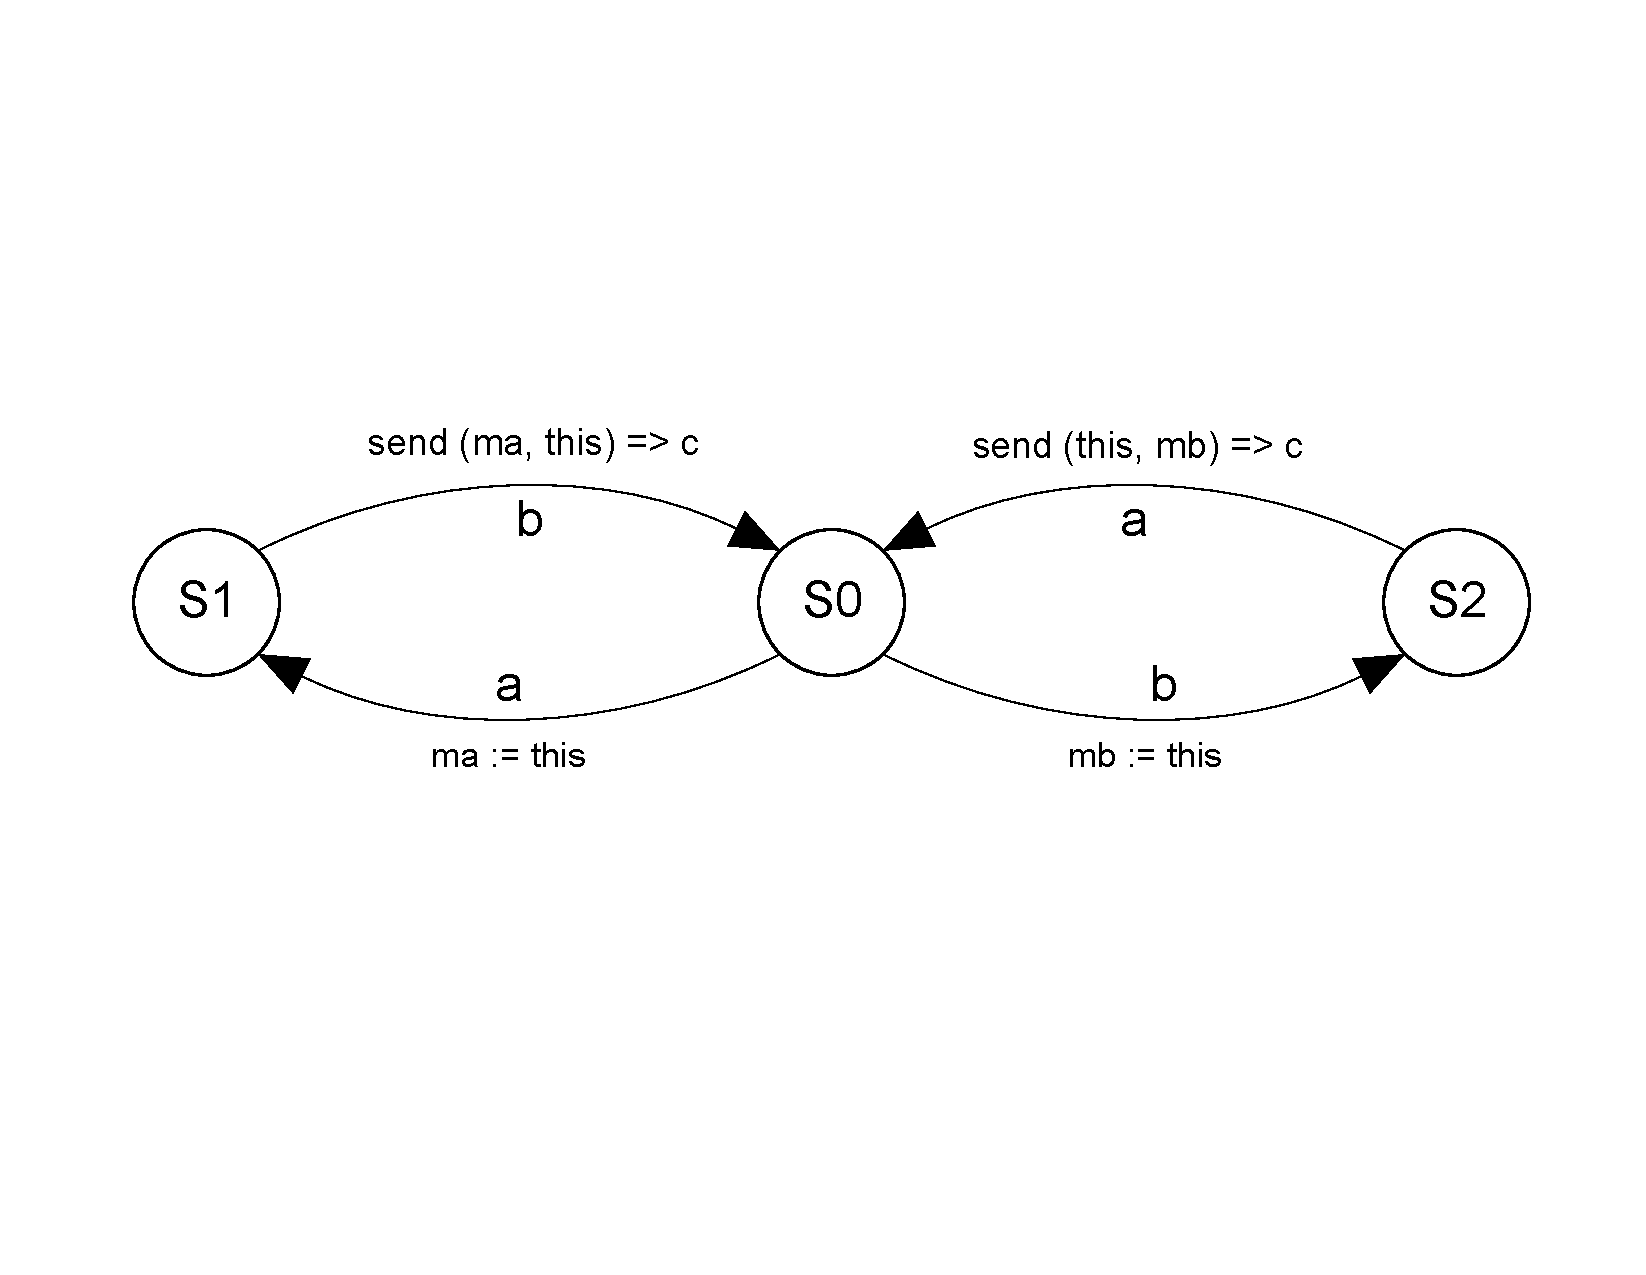
\includegraphics[scale=0.4]{figs/zip2.pdf}
  \caption{The transition diagram of the zip2 synchroniser.}
  \label{fig:zip2}
  \end{figure}

Mathematical model $S_{zip2} = (\Phi, \; \Pi)$, where
  \begin{itemize}
  \item[] $\Phi = (A, \; S, \; T)$,
    \begin{itemize}
    \item[] $C = (a, \; b)$, $P = (true)$, $A = C \times P = ((a, \; true), \: (b, \; true))$,
    \item[] $S = (s_{0}, s_{1}, s_{2})$, $s_{0}$ -- start state,
    \item[] $T$:
      \begin{tabular}{c|c|c|c}
      $A$ \textbackslash $S$ & $s_{0}$ & $s_{1}$ & $s_{2}$\\
      \hline
      $(a, \; true)$ & $s_{1}$ & $s_{1}$ & $s_{0}$\\
      \hline
      $(b, \; true)$ & $s_{2}$ & $s_{0}$ & $s_{2}$\\
      \end{tabular}
    \end{itemize}
  \item[] $\Pi \: : \: S \times \Omega \to V$,
    \begin{itemize}
    \item[] $\Omega = (c)$,
    \item[] $V = ((a, \; b), \: (b, \; a))$
    \end{itemize}
  \end{itemize}

An output message is emitted when a transition happens either from the state $s_{1}$ or the state $s_{2}$. These states are reached in two paths:
  \begin{itemize}
  \item[]
$W_{0} = ((s_{0}, \; a), \: (s_{1}, \; b))$

$\Pi \; (s_{1}, c) = \psi_{\sqcap} \; \{\mu_{0} = a \: | \: \rho_{10}^{c} \; (s_{0}) = 1, \mu_{1} = b \: | \: \rho_{11}^{c} \; (s_{1}) = 1\}$, $k = 1$, $i = 0,1$
  \item[]
$W_{1} = ((s_{0}, \; b), \: (s_{2}, \; a))$

$\Pi \; (s_{2}, c) = \psi_{\sqcap} \; \{\mu_{0} = b \: | \: \rho_{20}^{c} \; (s_{0}) = 1, \mu_{2} = a \: | \: \rho_{22}^{c} \; (s_{2}) = 1\}$, $k = 2$, $i = 0,2$ 
  \end{itemize}
  \end{enumerate}


\section{Synchroniser code}
The full grammar of the \ak\ synchroniser syntax is given in Appendix \ref{sync_syntax}. In this section we provide a detailed explaination of what every language construct mean.

Terminal symbols in the grammar are language keywords, special symbols, user-defined identifiers $\langle$id$\rangle$ and constant integers $\langle$const$\rangle$. The language keywords are \begin{bf}sync\end{bf}, \begin{bf}store\end{bf}, \begin{bf}state\end{bf}, \begin{bf}int\end{bf}, \begin{bf}enum\end{bf}, \begin{bf}on\end{bf}, \begin{bf}elseon\end{bf}, \begin{bf}else\end{bf}, \begin{bf}do\end{bf}, \begin{bf}send\end{bf}, \begin{bf}nil\end{bf}, \begin{bf}this\end{bf} and \begin{bf}goto\end{bf}. The special symbols are curved brackets \begin{bf}\{ \}\end{bf}, square brackets \begin{bf}[ ]\end{bf}, parantheses \begin{bf}( )\end{bf}, comma \begin{bf},\end{bf}, dot \begin{bf}.\end{bf}, semicolon \begin{bf}:\end{bf}, plus \begin{bf}+\end{bf}, minus \begin{bf}-\end{bf}, ampersand \begin{bf}\&\end{bf}, at sign \begin{bf}@\end{bf}, question mark \begin{bf}?\end{bf}, or \begin{bf}$||$\end{bf}, equal sign \begin{bf}=\end{bf} and arrow \begin{bf}$\Rightarrow$\end{bf}. A user-defined identifier is an ASCII string that follows the C conventions. Non-terminal symbol $\langle$int-exp$\rangle$ stands for integer expressions. The grammar for integer expression used in our implementation of a synchroniser compiler (Appendix \ref{int_exp_gr}) is a simplified version of the C grammar for arithmetic expression.


A synchroniser program consists of a heading $\langle$head$\rangle$ followed by the synchroniser's body wrapped in curved brackets.

The heading of a synchroniser program (Fig \ref{sync_syntax:head}) holds the synchroniser's name, optional configuration parameters $\langle$confs$\rangle$ and the communicating channel signature $\langle$params$\rangle$. The name is an ASCII string that follows the C convention. The name is specified after the keyword \begin{bf}sync\end{bf}.

The configuration parameters are integer constants introduced to avoid trivially altered synchroniser programs. They are specified in square brackets before the channel signature. An example of a configurable counter synchroniser can be found in \cite{astrakahn}.

\begin{figure}[h!]
\small
\begin{grammar}
[(colon){$\rightarrow$}]
[(semicolon)$|$]
[(comma){}]
[(period){\\}]
[(quote){\begin{bf}}{\end{bf}}]
[(nonterminal){$\langle$}{$\rangle$}]
<synchroniser>:<head>,"\{"<decls>,<trans>"\}".
<head>:"sync", <id>, [<confs>],<params>.

<confs>:"{\tt [}",<conf>,[",", <conf>]*,"{\tt ]}".
<conf>:<id>
\end{grammar}
\caption{Heading of the synchroniser and the configuration parameters}
\label{sync_syntax:head}
\end{figure}

The channel signature $\langle$params$\rangle$ (Fig. \ref{sync_syntax:params}) defines the input channels $\langle$inparam$\rangle$ and the output channels $\langle$outparam$\rangle$ of the synchroniser and their bracketing depths. The input channels are required to have the bracketing depths $\langle$indepth$\rangle$, while the output channels are guaranteed to have the bracketing depths specified with depth expressions $\langle$depth-exp$\rangle$. The depth expressions can be controlled by the configuration parameters. Output channels with the depth $-1$ are not sent any data to them and input channels with the depth $-1$ are ignored in the synchroniser program.

\begin{figure}[h!]
\small
\begin{grammar}
[(colon){$\rightarrow$}]
[(semicolon)$|$]
[(comma){}]
[(period){\\}]
[(quote){\begin{bf}}{\end{bf}}]
[(nonterminal){$\langle$}{$\rangle$}]
<params>:"(",[<inparam>,[",", <inparam>]*],"{\tt |}",[<outparam>,[",", <outparam>]*],")"
\end{grammar}
\end{figure}

\begin{figure}[h!]
\small
\begin{grammar}
[(colon){$\rightarrow$}]
[(semicolon)$|$]
[(comma){}]
[(period){\\}]
[(quote){\begin{bf}}{\end{bf}}]
[(nonterminal){$\langle$}{$\rangle$}]
<inparam>:<chan>,[":",<indepth>].
<chan>:<id>.
<indepth>:<var> ; <const>.

<outparam>:<chan>,[":",<depth-exp>].
<depth-exp>:<const> ; <var> ; <var>,"{\tt+}",<shift> ; <var>,"{\tt -}",<shift>.
<shift>:<const> ; <conf>.

<var>:<id>
\end{grammar}
\caption{Channel signature of the synchroniser}
\label{sync_syntax:params}
\end{figure}

The synchroniser's body includes store and state variable declarations $\langle$decls$\rangle$ followed by the definitions of transitions between states $\langle$trans$\rangle$.

Store variables are the storage mechanism \ak\ provides to synchronisers. A store variable is capable of storing a data message or a tail of a message from the associated channel $\langle$chan$\rangle$ (Fig. \ref{sync_syntax:decls}). (TODO: what is a tail and how is it used?) State variables are either integers of the size $\langle$const$\rangle$ or enumerations. (TODO: how does enum work?)

(TODO:) Tail names can be used in declaration of store variables in the same manner as channel names. A store variable can be assigned messages from several channels: x : foo,bar, in which case it is assumed that the variable has the least common type that the channels can be coerced up to. (TODO: fix the grammar for it)

\begin{figure}[h!]
\small
\begin{grammar}
[(colon){$\rightarrow$}]
[(semicolon)$|$]
[(comma){}]
[(period){\\}]
[(quote){\begin{bf}}{\end{bf}}]
[(nonterminal){$\langle$}{$\rangle$}]
<decls>:[<store-decl> ; <state-decl>]*.

<store-decl>:"store", <id>,"{\tt :}",<chan-tail>[",", <id>,"{\tt :}",<chan-tail>]*.
<chan-tail>:<chan> ; <tail>.
<tail>:<id>.

<state-decl>:"state", <type>,<id>[",", <id>]*.
<type>:"int(",<const>,")" ; "enum(",<id>,[",", <id>]*,")"
\end{grammar}
\caption{Store and state variable declarations.}
\label{sync_syntax:decls}
\end{figure}

Transitions of the synchroniser define which channels are read and in what order. The on-clause defines the condition on which the transition takes place. The do-clause is a list of actions that evaluate the functional. The send-clause forms and sends the output messages. The goto-clause defines the state transition (Fig. \ref{sync_syntax:trans}).

\begin{figure}[h!]
\small
\begin{grammar}
[(colon){$\rightarrow$}]
[(semicolon)$|$]
[(comma){}]
[(period){\\}]
[(quote){\begin{bf}}{\end{bf}}]
[(nonterminal){$\langle$}{$\rangle$}]
<trans>:<tran>[",", <tran>]*.
<tran>:[<label>,":"],[<on-clause>],[<do-clause>],[<send-clause>],[<goto-clause>].

<goto-clause>:"goto", <label>
\end{grammar}
\caption{Transitions and goto-clause of the synchroniser}
\label{sync_syntax:trans}
\end{figure}

Whether a transition takes place depends on the channel status and optionally the content of the messages (Fig. \ref{sync_syntax:on}). The state transitions of a synchroniser can depend on the content of the current message but never on that of a stored one.

The channel name $\langle$chan$\rangle$ on its own stands for the availability predicate for the corresponding channel, i.e. the condition that a message of any kind is available.

The condition $\langle$chan$\rangle$\begin{bf}.else\end{bf} is equivalent to $\langle$chan$\rangle$ except it is tested after any other condition involving the channel. Although several different channels can be tested in any given state, once a test has established the readiness of a channel, the synchroniser is committed, hence the set of conditions applied to the message on any input channel $\langle$chan$\rangle$ must be exhaustive. If it is not, the final clause \begin{bf}on\end{bf} $\langle$chan$\rangle$\begin{bf}.else;\end{bf} is assumed. That clause discards the input message and transitions the synchroniser back to its current state.

A channel carries a stream that consists of messages and possibly segmentation marks. The synchroniser detects a segmentation mark of the depth $\langle$id$\rangle$ with the channel condition \begin{bf}on\end{bf} $\langle$chan$\rangle${\tt .@}$\langle$id$\rangle$. 

When a message is received on a channel, it can be matched with a pattern $\langle$pattern$\rangle$ in order to extract parameters needed to select a specific transition. (TODO: what is a tail and how is it used?) To support message formats where several variants of a message are possible, a qualifier \begin{bf}?\end{bf}$\langle$id$\rangle$ is available as an input condition. It qualifies input messages as belonging to the $\langle$id$\rangle$ variant.

(TODO: how does elseon-clause behave?)

\begin{figure}[h!]
\small
\begin{grammar}
[(colon){$\rightarrow$}]
[(semicolon)$|$]
[(comma){}]
[(period){\\}]
[(quote){\begin{bf}}{\end{bf}}]
[(nonterminal){$\langle$}{$\rangle$}]
<on-clause>:"on", <chan-cond> ; "elseon", <chan-cond>.
<chan-cond>:<chan>,[".else" ; ".","{\tt @}",<id> ; ".?",<id> ; ".",["?",<id>]<pattern>]["{\tt \&}"<guard-exp>].
<pattern>:"(",<id>,[",", <id>]*,["{\tt ||}",<tail>],")".
<guard-exp>:<int-exp>
\end{grammar}
\caption{On-clause of the synchroniser}
\label{sync_syntax:on}
\end{figure}

TODO: data expression (Fig. \ref{sync_syntax:do})
( ) denotes the concatenation of the messages it is subject to.
A message received on a channel can be referred to by the keyword 'this'.


\begin{figure}[h!]
\small
\begin{grammar}
[(colon){$\rightarrow$}]
[(semicolon)$|$]
[(comma){}]
[(period){\\}]
[(quote){\begin{bf}}{\end{bf}}]
[(nonterminal){$\langle$}{$\rangle$}]
<data-exp>:<primary-mes> ; "(",<primary-mes>,["," <primary-mes>]*,")".
<primary-mes>:<var> ; <var>=<int-exp> ; "this".

<do-clause>:"do", <assign>,[",", <assign>]*.
<assign>:<id>,"{\tt :=}",<int-exp> ; <id>,"{\tt :=}",<data-exp>
\end{grammar}
\caption{Data expression and do-clause of the synchroniser}
\label{sync_syntax:do}
\end{figure}

The send-clause (Fig. \ref{sync_syntax:send})

\begin{figure}[h!]
\small
\begin{grammar}
[(colon){$\rightarrow$}]
[(semicolon)$|$]
[(comma){}]
[(period){\\}]
[(quote){\begin{bf}}{\end{bf}}]
[(nonterminal){$\langle$}{$\rangle$}]
<send-clause>:"send", <dispatch>,[",", <dispatch>]*.
<dispatch>:<msg-exp>,"{\tt =>}",<chan>.
<msg-exp>:"{\tt @}",<int-exp> ; "?",<id> ; ["?",<id>],<data-exp> ; "nil"
\end{grammar}
\caption{Send-clause of the synchroniser}
\label{sync_syntax:send}
\end{figure}


\section{Execution order of synchroniser\label{execod}}
Algorithm of the execution of synchronisers, in which order transitions execute


\section{The implementation of the compiler}
The implementation of the compiler frontend in OCaml \cite{realworldocaml}, with code generation to a python structure.

  \subsection{Type checking}
  \subsection{Synchroniser passport}
%  \subsection{Dead code elimination}
%Based on Section \ref{execod}.
